\documentclass[11pt,a4paper]{article}
\usepackage[T1]{fontenc}
\usepackage[utf8]{inputenc}
\usepackage{lmodern}
\usepackage[english]{babel}
\usepackage[a4paper,margin=2.2cm]{geometry}
\usepackage{graphicx,booktabs,array,microtype}
\usepackage[hidelinks]{hyperref}
\setlength{\parskip}{3pt}
\setlength{\parindent}{0pt}
\newcommand{\sect}[1]{\par\medskip\noindent\textbf{\large #1}\par\smallskip}
\begin{document}
\begin{center}
{\Large\bfseries GroundOne: A Specialist Decision Model for Groundedness Verification\\ in Local Retrieval-Augmented Generation}\\[6pt]
{\normalsize Francesco Pio De Dominicis \quad·\quad Supervisor: Prof.\ Paolo Garza\\
Master's Degree in Computer Engineering, Politecnico di Torino, A.Y. 2025/2026}\\[4pt]
\textit{Thesis summary}
\end{center}

\sect{Motivation}
Retrieval-augmented generation (RAG) gives language models access to private documents, and the whole pipeline can now
run on a consumer device, which helps privacy, offline use and cost. Retrieval does not remove hallucinations: answers
still contain sentences that the retrieved context does not support or contradicts. Detecting them must happen on every
answer, on the same resource-limited machine that hosts the generator. Locality has a precise technical consequence: on
a single device reading text is cheap and writing it is expensive. The model reads its input in one forward pass,
bounded by compute, but writes one token at a time, each bounded by the memory bandwidth needed to read all the weights;
on the laptop used in this thesis a written token costs fourteen to sixteen times more than a read one, and a survey of
current local hardware shows the same asymmetry everywhere. Verifiers today are either small encoders, which return one
fixed score per document–sentence pair, or LLM judges, which write their verdicts token by token and often break
the output format. A third family, \emph{decision models}, answers closed questions in one forward pass by reading the
probability of each answer option from the logits. Whether a compact decision model specialised in a single task can
match LLM judges and encoders, where its advantage comes from, and whether its probabilities are usable, had not been studied
in a controlled way on consumer hardware.

\sect{GroundOne}
GroundOne is a decision model specialised in one decision: for every sentence of a RAG answer, does the retrieved document
support it, contradict it, or not mention it? A marker follows every sentence, and the verdicts of all $K$ sentences are
read from the logits of three answer letters at the markers, in a single forward pass, without generating any text
(Figure~\ref{fig:prompt}). Qwen2.5 models with 0.5B and 3B parameters are fine-tuned with LoRA on the human-annotated
answers of RAGTruth, with a class-weighted loss restricted to the three letters. A temperature and a per-class bias fitted
on the dev set calibrate the probabilities, and a threshold chosen on the same data turns them into labels that agree with
the probabilities shown to the user. Everything, from dataset construction to training, evaluation and serving, runs on
one Apple M4 laptop with 16\,GB of memory, with MLX and no external service.

\begin{figure}[h]
\centering
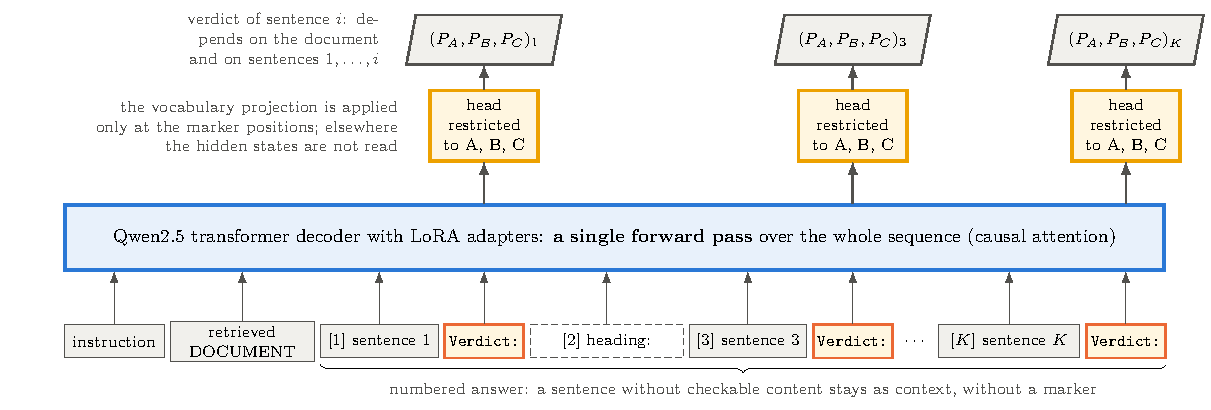
\includegraphics[width=0.86\textwidth]{../Thesis/images/diagrams/method_marked_prompt_tikz.pdf}
\caption{GroundOne's marked prompt: the verdicts of all sentences are read at the \texttt{Verdict:} markers in one
forward pass.}
\label{fig:prompt}
\end{figure}

\sect{Data and experimental setup}
No label was annotated anew: RAGTruth's span annotations were converted into a three-way label per sentence with rules
fixed in advance. Three test sets were built, checked and frozen before any training, with leakage controlled at document
level: the RAGTruth test split (T1, 17{,}284 sentences), LLM-AggreFact (T2, eleven datasets) and VitaminC (T3, an
out-of-domain fact-checking test). GroundOne is compared with cues that never read the document, the untrained models,
LLM judges of the same size with and without probabilities, two generalist decision models (Rizzo-Flow, 4B, and
d1-3B of Liquid AI) and specialised encoders (MiniCheck-RoBERTa, HHEM), all on the same machine, with intervals from a
cluster bootstrap.

\sect{Results}
Specialisation works in the domain it targets (Table~\ref{tab:results}). On T1 GroundOne reaches a three-way balanced
accuracy of 0.769 (0.5B) and 0.832 (3B), against 0.37 and 0.44 before training; its AUROC (0.905 and 0.940) exceeds that
of the encoders (about 0.82), and in three-way balanced accuracy it clearly beats both generalist decision models. On
LLM-AggreFact the 3B is on par with MiniCheck-RoBERTa (74.8 against 74.0, interval including zero). On VitaminC the gain
disappears, and d1-3B is much stronger: a specialist is not a general fact-checking tool. The readout matters by itself:
with the same trained model, choosing among the three admissible letters is more accurate than letting the model generate
its verdict (+0.25 for the 0.5B, +0.07 for the 3B), at the same latency. On answers of fourteen or more sentences
GroundOne is 1.7 to 2 times faster than a terse LLM judge and about six times faster than a verbose one, always with a valid output; net of reading the text, which all approaches pay, it decides 18 to 33 times faster than the terse LLM judge; if the document is already in the KV cache, as when a rewritten answer is verified, the overall advantage rises to 3.4 to 3.6 times. It uses less energy (5.5 and 33 joules per answer on average), although the saving is smaller than the time
saving because a long prefill draws more power than decoding. After calibration the Expected Calibration Error of the 3B
on T1 is 0.019, while LLM judges asked for the same output give probabilities that barely separate right from wrong
decisions. The whole evaluation runs with no network access and bit-identical results, 8-bit weights cost no accuracy
against bf16, and generator and verifier fit together in one process with a 6.1\,GB peak.

\begin{table}[h]
\centering
\small
\begin{tabular}{>{\raggedright\arraybackslash}p{7.2cm}cc}
\toprule
Measure & GroundOne 0.5B & GroundOne 3B \\
\midrule
T1 three-way balanced accuracy (untrained) & 0.769 (0.37) & 0.832 (0.44) \\
T1 AUROC of P(supported) (best encoder 0.82) & 0.905 & 0.940 \\
T2 macro balanced accuracy (MiniCheck-RoBERTa 74.0) & 70.1 & 74.8 \\
Readout vs generated verdict, same weights & +0.25 & +0.07 \\
Speed-up at $K \geq 14$ vs terse / verbose LLM judge & 1.95$\times$ / 6.2$\times$ & 1.73$\times$ / 6.2$\times$ \\
Time and energy per answer & 0.41\,s, 5.5\,J & 2.57\,s, 33\,J \\
\bottomrule
\end{tabular}
\caption{Main results. Times are for answers with fourteen or more sentences; energy is the average per answer; the untrained 3B was evaluated on 600 T1 answers.}
\label{tab:results}
\end{table}

\sect{GroundOne Studio: a local application and a case study}
A native macOS application, written in Swift with MLX Swift, puts the verifier to work in a complete RAG assistant in which
retrieval (SQLite full-text search and small embeddings), generation (Qwen2.5-3B, 4-bit), verification and a local
LLM judge share one process, with at most 6.9\,GB of memory and no network. A conformance test on 200 T1 answers
shows identical tokens and probabilities within 0.005 of the Python implementation for the 3B. The generator's native
answer is shown first; the user can then verify it with GroundOne alone or together with the LLM judge, inspect the
probabilities and the supporting passage of each sentence, and have flagged or selected sentences rewritten from the
sources, one short request per sentence and by error type. In a case study with 100 injected errors GroundOne flags the
error in 97 of the 98 answers in which the sentence receives a verdict, the LLM judge in 84, and targeted rewriting lowers the
answers still containing the error from 100\,\% to 6\,\%: changed numbers and dates are mostly restored from the source,
fabricated sentences deleted. Repeating the study with the 0.5B shows why the three-way verdict matters: it labels changed
values as not mentioned rather than contradicted, and the generator then deletes them instead of correcting them. These
answers are accepted by GroundOne, not independently verified.

\sect{Limitations and future work}
The main limits are the narrow training data, through which contradictions outside data-to-text and hallucinations hidden
in otherwise copied sentences are learnt only in part, a training recipe not fully robust to the seed, a single platform
and model family, and English-only data. Future work includes a more robust recipe (bias correction, gradient clipping,
several seeds), training data with paraphrased support and minimal edits, a llama.cpp port to measure other hardware,
per-language adapters, attribution of each verdict to a passage, a larger generator and an independent check of rewritten
sentences in the application.
\end{document}
